\subsection{正规方程法}
\label{sec:ls-normal-equations-method}

\subsubsection{主要思想}

现在转向超定的最小二乘问题：输入满列秩的$\bm A\in\mathbb R^{m\times d}$（$m\geq d$）和$\bm b\in\mathbb R^m$，求唯一的最小二乘解$\hat{\bm x}$。第~\ref{sec:ls-ordinary-ls}节已经证明，这一目标等价于正规方程$\bm A^\top\bm A\hat{\bm x}=\bm A^\top\bm b$（式~\eqref{eq:linear-algebra-normal-equations}）。满列秩时系数矩阵$\bm A^\top\bm A$对称正定，于是$m\times d$的最小二乘问题变成一个$d$阶正定方程，可以直接交给第~\ref{sec:ls-cholesky}节的Cholesky分解求解。

\subsubsection{算法实现}

\paragraph{形成Gram矩阵}
第一步形成Gram矩阵$\bm G=\bm A^\top\bm A$与右端$\bm c=\bm A^\top\bm b$。把$\bm A$按行写开，二者都是各行贡献之和：先令$\bm G=\bm0$、$\bm c=\bm0$，再对$i=1,\ldots,m$依次累加
\[
 \bm G\leftarrow\bm G+\bm A_{i,:}^\top\bm A_{i,:},\qquad
 \bm c\leftarrow\bm c+b_i\bm A_{i,:}^\top .
\]
每读入一行就能完成它的贡献，不必同时保存所有观测行；$\bm G$对称，只需累加下三角部分。

\paragraph{\texorpdfstring{$\bm L\bm L^\top$}{LL\textasciicircum T}分解}
然后用第~\ref{sec:ls-cholesky}节的逐列过程计算$\bm G=\bm L\bm L^\top$。这一步要求$\bm G$正定，满列秩恰好保证了这一点：对任意$\bm z\neq\bm0$有$\bm A\bm z\neq\bm0$，所以$\bm z^\top\bm G\bm z=\lVert\bm A\bm z\rVert_2^2>0$。

\paragraph{前代与回代}
有了因子，先用第~\ref{sec:ls-lu}节的前代求解$\bm L\bm y=\bm c$，再用回代求解$\bm L^\top\hat{\bm x}=\bm y$，得到最小二乘解$\hat{\bm x}$。两次三角求解的次序来自$\bm L(\bm L^\top\hat{\bm x})=\bm c$，与用Cholesky分解解正定方程的步骤相同。第~\ref{sec:ls-direct-method-comparison}节在直线拟合数据上给出了这三步的数值。

\subsubsection{算法分析}

\paragraph{正确性}
两次三角求解给出$\bm L\bm L^\top\hat{\bm x}=\bm c$，即$\bm A^\top\bm A\hat{\bm x}=\bm A^\top\bm b$，所以$\hat{\bm x}$满足正规方程，由定理~\ref{thm:ls-least-squares-solutions}是唯一的最小二乘解。

\paragraph{数值敏感度}
这条路线的代价在精度。对满列秩矩阵定义$\kappa_2(\bm A)=\sigma_{\max}(\bm A)/\sigma_{\min}(\bm A)$，方阵时它与第~\ref{sec:ls-matrix-condition-number}节的定义一致。

\begin{theorem}[正规方程使条件数平方]
\label{thm:ls-normal-equations-condition-squaring}
设$\bm A\in\mathbb R^{m\times d}$满列秩，则$\kappa_2(\bm A^\top\bm A)=\kappa_2(\bm A)^2$。
\end{theorem}
\begin{proof}
由第~\ref{sec:ls-svd}节的奇异值分解$\bm A=\bm U\bm\Sigma\bm V^\top$，得
\[
 \bm A^\top\bm A=\bm V\operatorname{diag}(\sigma_1^2,\ldots,\sigma_d^2)\bm V^\top .
\]
满列秩时$\sigma_d>0$，这是对称正定矩阵的谱分解，其最大、最小特征值即最大、最小奇异值，分别为$\sigma_1^2$与$\sigma_d^2$，故$\kappa_2(\bm A^\top\bm A)=\sigma_1^2/\sigma_d^2=\kappa_2(\bm A)^2$。
\end{proof}

$\bm A$压缩得很厉害的方向在$\bm G$中被压缩两次，形成$\bm G$时的舍入就可能抹掉这些方向上的信息，误差界随之带上$\kappa_2(\bm A)^2$（第~\ref{sec:ls-ls-regularization-sensitivity}节）。

\paragraph{计算代价与适用范围}
形成Gram矩阵可能增加填充：$\bm A$只要有一行全是非零元，这一行的外积就使$\bm G$成为稠密矩阵。稠密情形下形成$\bm G$约需$md^2$次运算，分解约需$d^3/3$次，总工作为$O(md^2+d^3)$。秩亏时正规方程仍刻画全部最小二乘解，但$\bm G$只是半正定的，Cholesky分解会遇到零主元，本算法的前提不再成立；这时的选解由第~\ref{sec:ls-svd-solve}节的SVD路线完成。

\subsection{QR求解}
\label{sec:ls-qr-method}

正规方程法的精度损失来自形成$\bm A^\top\bm A$。QR求解不形成它，而是直接对$\bm A$作正交三角化。下面先利用QR因子写清最小二乘与满行秩最小范数解的共同求解过程，再分别说明修正Gram--Schmidt、Householder反射与Givens旋转怎样计算这些因子。

\subsubsection{主要思想}

输入满列秩的$\bm A\in\mathbb R^{m\times d}$（$m\geq d$）和$\bm b\in\mathbb R^m$，求唯一的最小二乘解$\hat{\bm x}$。正交变换保持欧氏长度，用它同时变换$\bm A$和$\bm b$不会改变残差的长度。因此可以找一个正交矩阵把$\bm A$化为上三角形，最小二乘问题就变成一个三角方程，全程不必形成$\bm A^\top\bm A$。先写清共同的求解步骤，正交因子的计算留给后面三个小节。

\subsubsection{算法实现}

\paragraph{QR分解}
第一步计算QR分解。第~\ref{chap:normed-inner-product-spaces}章的薄QR分解（式~\eqref{eq:ls-qr-factorization}）给出$\bm A=\bm Q_1\bm R$；把$\bm Q_1$的列补成$\mathbb R^m$的标准正交基，新增的列排成$\bm Q_2$，就得到
\[
 \bm A=\bm Q\begin{bmatrix}\bm R\\\bm0\end{bmatrix},\qquad \bm Q=[\bm Q_1\;\bm Q_2],
\]
其中$\bm Q$为$m$阶正交矩阵，$\bm R$为$d$阶可逆上三角矩阵。实际完成这一步的是后面三种方法；反射和旋转只需记录各步变换，不必显式形成$\bm Q$。

\paragraph{变换右端}
然后对右端施加相同的正交变换，计算
\[
 \bm Q^\top\bm b=\begin{bmatrix}\bm c_1\\\bm c_2\end{bmatrix},
\]
其中$\bm c_1$含前$d$个分量。回代只需要$\bm c_1=\bm Q_1^\top\bm b$，所以使用薄正交基$\bm Q_1$时只算这一部分；修正Gram--Schmidt中$\bm c_1$的具体计算顺序在第~\ref{sec:ls-mgs}节说明。

\paragraph{求解\texorpdfstring{$\bm R\hat{\bm x}=\bm c_1$}{Rx=c1}}
最后用回代求解$\bm R\hat{\bm x}=\bm c_1$，得到最小二乘解$\hat{\bm x}$。

\paragraph{欠定情形：转置QR}
同一种分解也能处理欠定方程。设$\bm A\in\mathbb R^{m\times d}$满行秩，$m<d$，输入仍为$\bm A$、$\bm b$，求解目标改为第~\ref{sec:ls-select-among-solutions}节的最小范数精确解$\bm x_\star$。由于$\bm x_\star$应位于$\operatorname{range}(\bm A^\top)$中，这时把分解用于$\bm A^\top$，而不是$\bm A$。先计算薄QR分解$\bm A^\top=\bm Q\bm R$，其中$\bm Q\in\mathbb R^{d\times m}$的列标准正交，$\bm R$为$m$阶可逆上三角矩阵，于是$\bm A=\bm R^\top\bm Q^\top$。再用前代求解下三角方程$\bm R^\top\bm y=\bm b$，得到$\bm x_\star$在行空间基$\bm Q$下的坐标$\bm y$，最后计算$\bm x_\star=\bm Q\bm y$。先解$\bm A\bm A^\top\bm z=\bm b$再取$\bm A^\top\bm z$也得到同一个解，但要先形成Gram矩阵$\bm A\bm A^\top$，转置QR避免了这一步。

\subsubsection{算法分析}

\paragraph{正确性}
两个分支的正确性合写成下面的定理。

\begin{theorem}[QR给出最小二乘解与最小范数解]
\label{thm:ls-qr-least-squares}
设$\bm A\in\mathbb R^{m\times d}$，$\bm b\in\mathbb R^m$。
\begin{enumerate}
 \item 设$\bm A$满列秩，$\bm A=\bm Q\left[\begin{smallmatrix}\bm R\\\bm0\end{smallmatrix}\right]$，$\bm Q^\top\bm b=\left[\begin{smallmatrix}\bm c_1\\\bm c_2\end{smallmatrix}\right]$。则$\hat{\bm x}=\bm R^{-1}\bm c_1$是唯一的最小二乘解，最小残差范数为$\lVert\bm c_2\rVert_2$。
 \item 设$\bm A$满行秩，$\bm A^\top=\bm Q\bm R$为薄QR分解，$\bm R^\top\bm y=\bm b$。则$\bm x_\star=\bm Q\bm y$是$\bm A\bm x=\bm b$唯一的最小范数解。
\end{enumerate}
\end{theorem}
\begin{proof}
(1) 正交变换保持长度，对任意$\bm x$有
\begin{equation}
 \begin{aligned}
 \lVert\bm A\bm x-\bm b\rVert_2^2
 &=\lVert\bm Q^\top(\bm A\bm x-\bm b)\rVert_2^2\\
 &=\lVert\bm R\bm x-\bm c_1\rVert_2^2+\lVert\bm c_2\rVert_2^2 .
 \end{aligned}
 \label{eq:ls-qr-residual-split}
\end{equation}
第二项与$\bm x$无关；$\bm R$可逆，第一项当且仅当$\bm x=\bm R^{-1}\bm c_1$时为零。

(2) $\bm A\bm x_\star=\bm R^\top\bm Q^\top\bm Q\bm y=\bm R^\top\bm y=\bm b$，并且$\bm x_\star\in\operatorname{range}(\bm Q)=\operatorname{range}(\bm A^\top)=(\ker\bm A)^\perp$。任何其他解都与$\bm x_\star$相差$\ker\bm A$中的非零向量，由勾股关系范数更大。
\end{proof}

\paragraph{数值敏感度}
数值上要区分两个来源：最小二乘问题本身对数据的敏感度由问题决定（第~\ref{sec:ls-ls-regularization-sensitivity}节），计算QR因子时引入多少误差则取决于所用的正交化过程。三种实现的稳定性并不相同，下面分别说明。

\paragraph{秩亏情形}
秩亏时$\bm R$出现零对角元，不能照搬可逆$\bm R$的回代，最小范数最小二乘解按第~\ref{sec:ls-svd-solve}节用SVD求解。带列主元的QR能把线性无关的主元列排到前面，但只取主元变量回代、把其余原坐标置零，一般得到的是基本解，不能据此认定它是最小范数解。所以一般秩的情形本节统一使用SVD路线。

\subsubsection{修正GS}
\label{sec:ls-mgs}

\term{修正Gram--Schmidt}（modified Gram--Schmidt）处理满列秩的$\bm A\in\mathbb R^{m\times d}$（$m\geq d$）。它与第~\ref{chap:normed-inner-product-spaces}章的Gram--Schmidt正交化只差一处：扣除旧方向上的分量时，每次对当前剩余向量作投影，扣除后再计算下一个投影，而不是都用原始列计算内积。所得QR因子用于同一个输入$\bm A$、$\bm b$的最小二乘求解，输出仍为$\hat{\bm x}$。

\paragraph{逐列正交化}
先令$\bm R=\bm0$，再按$j=1,\ldots,d$依次处理各列。第$j$列令$\bm u=\bm a_j$，这里$\bm a_j$表示$\bm A$的第$j$列；然后按$i=1,\ldots,j-1$依次执行
\[
 r_{i,j}=\bm q_i^\top\bm u,\qquad \bm u\leftarrow\bm u-r_{i,j}\bm q_i .
\]
每次内积用的是刚更新过的剩余向量，而不是原始列$\bm a_j$。扣除全部旧方向后，取$r_{j,j}=\lVert\bm u\rVert_2$、$\bm q_j=\bm u/r_{j,j}$，这一列就完成了，接着处理下一列。满列秩保证精确算术下$r_{j,j}>0$。全部列完成后，得到$\bm Q_1=[\bm q_1,\ldots,\bm q_d]$与上三角的$\bm R$。

\paragraph{变换右端与回代}
然后把右端当作额外的一列：令$\bm s=\bm b$，按$i=1,\ldots,d$依次计算$c_i=\bm q_i^\top\bm s$与$\bm s\leftarrow\bm s-c_i\bm q_i$，得到$\bm c=(c_1,\ldots,c_d)^\top$。这一顺序与前面的逐次投影一致；有限精度下$\bm Q_1$的列不完全正交，不宜把它直接换成另算$\bm Q_1^\top\bm b$。最后用回代求解$\bm R\hat{\bm x}=\bm c$，输出$\hat{\bm x}$。$\bm Q_1$、$\bm R$和剩余向量都只是内部状态。

\paragraph{正确性}
精确算术中各$\bm q_i$两两正交，所以对剩余向量和对原始列计算的内积相同：$\bm q_i^\top(\bm a_j-\sum_{k<i}r_{k,j}\bm q_k)=\bm q_i^\top\bm a_j$。修正形式因而给出与原来相同的QR分解，由定理~\ref{thm:ls-qr-least-squares}得到最小二乘解。

\paragraph{数值正交性与计算代价}
有限精度下，近相关的列扣除旧方向后剩余向量很短，其中舍入误差的相对影响被放大，算出的$\bm q_j$会偏离正交，必要时可以对$\bm u$再正交化一遍。检查结果时用$\lVert\bm Q_1^\top\bm Q_1-\bm I\rVert$衡量正交性，用$\lVert\bm A-\bm Q_1\bm R\rVert$衡量重构质量，二者要分开看。主要工作约为$2md^2$次运算。

\subsubsection{Householder}
\label{sec:ls-householder}

对满列秩的$\bm A\in\mathbb R^{m\times d}$（$m\geq d$），Householder方法逐列用正交反射消去对角元下方的元素，同时变换右端，最后调用三角回代。\term{Householder反射}（Householder reflection）$\bm H=\bm I-2\bm v\bm v^\top/(\bm v^\top\bm v)$把$\bm v$方向的分量变号，保持与$\bm v$正交的分量不变，是关于以$\bm v$为法向的超平面的镜面反射。只要选好$\bm v$，就能把当前列段反射到第一个坐标轴上，如图~\ref{fig:ls-householder-reflection}所示。以下保持原列顺序。

\begin{figure}[htbp]
  \centering
  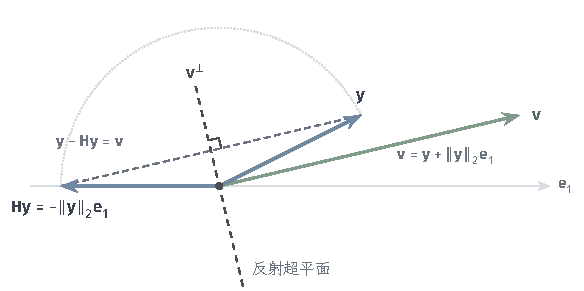
\includegraphics[width=98.94mm]{figures/01-basic-mathematics/03-vectors-matrices-and-multivariate-functions/tikz/c5-householder-reflection/figure.pdf}
  \caption{Householder反射的几何。取$\bm y=(2,1)^\top$，按式~\eqref{eq:ls-householder}令$\bm v=\bm y+\sqrt5\,\bm e_1$。反射超平面$\bm v^\perp$是$\bm y$与$\bm H\bm y=-\sqrt5\,\bm e_1$连线的垂直平分线，两者之差恰为$\bm v$；点线圆弧表示反射保持长度。解析式构造。}
  \label{fig:ls-householder-reflection}
\end{figure}

\paragraph{构造反射向量}
先令工作矩阵$\bm F=\bm A$、工作右端$\bm c=\bm b$。第$k$步取当前列段$\bm y=\bm F_{k:m,k}$，$y_1\geq0$时令$s=1$，$y_1<0$时令$s=-1$，构造
\begin{equation}
 \bm v=\bm y+s\lVert\bm y\rVert_2\bm e_1,\qquad
 \bm H=\bm I-\frac{2\bm v\bm v^\top}{\bm v^\top\bm v}.
 \label{eq:ls-householder}
\end{equation}
由下面的引理，$\bm H\bm y=-s\lVert\bm y\rVert_2\bm e_1$，该列下方的元素被消去。图~\ref{fig:ls-householder-reflection}中，$\bm y$与它的像$\bm H\bm y$关于超平面$\bm v^\perp$对称，两者之差就是$\bm v$。$\bm y=\bm0$时本步取恒等变换。

\paragraph{作用于剩余子块}
然后把同一个$\bm H$作用于剩余子块$\bm F_{k:m,k:d}$的各列和右端$\bm c_{k:m}$，每个向量都按
\[
 \bm z\mapsto\bm z-\frac{2\bm v(\bm v^\top\bm z)}{\bm v^\top\bm v}
\]
计算，只需一次内积和一次向量更新，不必形成整个反射矩阵；恒等变换时直接跳过。按$k=1,\ldots,d$重复上面两步。

\paragraph{回代}
最后取$\bm R=\bm F_{1:d,1:d}$，用回代求解$\bm R\hat{\bm x}=\bm c_{1:d}$，输出$\hat{\bm x}$。

\begin{example}[直线拟合的Householder三角化]
\label{ex:ls-householder-line-fit}
取示例~\ref{ex:ls-line-least-squares}的$\bm A=\left[\begin{smallmatrix}1&0\\1&1\\1&2\end{smallmatrix}\right]$、$\bm b=(1,2,2)^\top$。第一步$\bm y=(1,1,1)^\top$，$\lVert\bm y\rVert_2=\sqrt3$，$s=1$，$\bm v=(1+\sqrt3,1,1)^\top$，$\bm v^\top\bm v=6+2\sqrt3$。第一列变为$(-\sqrt3,0,0)^\top$；第二列$(0,1,2)^\top$与$\bm v$的内积为$3$，更新为$(-\sqrt3,\tfrac{\sqrt3-1}2,\tfrac{\sqrt3+1}2)^\top$；右端更新为$(-\tfrac5{\sqrt3},\tfrac1{\sqrt3},\tfrac1{\sqrt3})^\top$。三个向量的长度平方仍为$3$、$5$、$9$。

第二步作用于后两行，$\bm y=(\tfrac{\sqrt3-1}2,\tfrac{\sqrt3+1}2)^\top$，$\lVert\bm y\rVert_2=\sqrt2$，反射后$r_{2,2}=-\sqrt2$，右端后两分量变为$(-\tfrac1{\sqrt2},-\tfrac1{\sqrt6})^\top$。于是
\[
 \bm R=\begin{bmatrix}-\sqrt3&-\sqrt3\\0&-\sqrt2\end{bmatrix},\qquad
 \bm c_1=\Bigl(-\frac5{\sqrt3},-\frac1{\sqrt2}\Bigr)^{\!\top},
\]
回代得$\hat x_2=1/2$，$\hat x_1=5/3-1/2=7/6$，与示例~\ref{ex:ls-line-least-squares}一致；$\lvert c_3\rvert=1/\sqrt6$正是最小残差范数。$\bm R$与第~\ref{sec:ls-direct-method-comparison}节的Cholesky因子$\bm L^\top$只差各行的符号。
\end{example}

\paragraph{正确性}
单步消元的依据是下面的引理。

\begin{lemma}[Householder反射]
\label{lem:ls-householder-reflection}
设$\bm y\neq\bm0$，$\bm v$与$\bm H$由式~\eqref{eq:ls-householder}给出。则$\bm H$对称正交，且$\bm H\bm y=-s\lVert\bm y\rVert_2\bm e_1$。
\end{lemma}
\begin{proof}
$\bm H$显然对称；$\bm H^2=\bm I-4\bm v\bm v^\top/(\bm v^\top\bm v)+4\bm v(\bm v^\top\bm v)\bm v^\top/(\bm v^\top\bm v)^2=\bm I$，所以$\bm H^\top\bm H=\bm I$。由$s^2=1$与$sy_1=\lvert y_1\rvert$，
\[
 \bm v^\top\bm v=2\lVert\bm y\rVert_2^2+2\lVert\bm y\rVert_2\lvert y_1\rvert=2\bm v^\top\bm y>0,
\]
于是$\bm H\bm y=\bm y-\bm v=-s\lVert\bm y\rVert_2\bm e_1$。
\end{proof}

每个$\bm H$嵌入$m$阶后只作用于第$k$至$m$行；前$k-1$列在这些行上已经是零，反射后仍为零。所以旧的零结构保持不变，$d$步后$\bm F=\bm H_d\cdots\bm H_1\bm A$是上三角矩阵，$\bm c=\bm H_d\cdots\bm H_1\bm b$。这正是取$\bm Q^\top=\bm H_d\cdots\bm H_1$的QR分解，由定理~\ref{thm:ls-qr-least-squares}，回代所得即最小二乘解。

\paragraph{数值稳定性与计算代价}
符号$s$取与$y_1$相同，使$\bm v$的首分量是两个同号数相加；取相反符号时，$\bm y$接近$\bm e_1$方向会使$y_1-\lVert\bm y\rVert_2$严重相消。Householder QR后向稳定（第~\ref{sec:ls-numerical-stability}节），主要工作约为$2md^2-\tfrac23d^3$次运算。列主元可以辅助辨认近相关的列，但秩亏时的最小范数选择仍回到第~\ref{sec:ls-svd-solve}节。

\subsubsection{Givens}
\label{sec:ls-givens}

输入满列秩的$\bm A\in\mathbb R^{m\times d}$（$m\geq d$）和$\bm b\in\mathbb R^m$，求唯一的最小二乘解$\hat{\bm x}$。\term{Givens旋转}（Givens rotation）在两个坐标构成的平面内旋转，其余坐标不变；每次只混合两行，消去其中一个指定元素。逐列完成三角化后调用回代。由于只触及需要消去的元素，它适合对角线以下非零元很少的矩阵，以及在已有分解上新增观测行的情形。图~\ref{fig:ls-givens-householder-elimination}把旋转与反射并置。

\begin{figure*}[htbp]
  \centering
  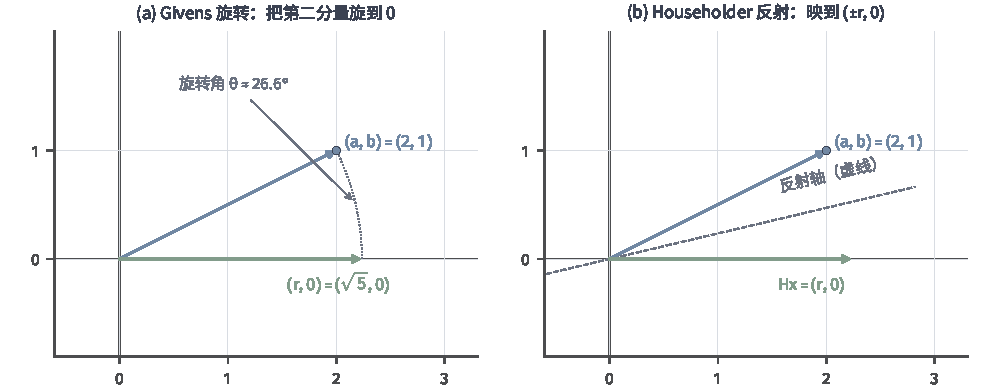
\includegraphics[width=168.998mm]{figures/00-shared/mathematical-preliminaries-upper/02-linear-spaces/matplotlib/ls-givens-householder-elimination/ls-givens-householder-elimination.pdf}
  \caption{两种初等正交消元。左：Givens旋转把$(a,b)=(2,1)^\top$沿圆弧旋到
  $(r,0)^\top$，$r=\sqrt5$，旋转角$\theta=\arctan(1/2)$；右：Householder反射沿角平分线
  把同一向量映到$(r,0)^\top$。两者都是正交变换，保持长度，区别在旋转（行列式$+1$）与
  反射（对称正交）。图中的反射取与式~\eqref{eq:ls-householder}相反的符号，精确算术中两种选择都可以。解析式教学构造。}
  \label{fig:ls-givens-householder-elimination}
\end{figure*}

\paragraph{消元顺序}
先令$\bm F=\bm A$、$\bm t=\bm b$，右端记作$\bm t$是为了不与旋转参数$c$混淆。按$k=1,\ldots,d$处理各列；在第$k$列中按$i=m,m-1,\ldots,k+1$自下而上消去$f_{i,k}$，每次使用相邻的第$i-1$、$i$两行。

\paragraph{构造旋转}
若$f_{i,k}=0$，直接跳过本次消元。否则令$\alpha=f_{i-1,k}$、$\beta=f_{i,k}$，计算
\begin{equation}
 \begin{gathered}
 \rho=\sqrt{\alpha^2+\beta^2},\qquad c=\alpha/\rho,\qquad s=\beta/\rho,\\
 \bm G=\begin{bmatrix}c&s\\-s&c\end{bmatrix},
 \end{gathered}
 \label{eq:ls-givens}
\end{equation}
于是$\bm G(\alpha,\beta)^\top=(\rho,0)^\top$。这里的$s$与Householder反射中的符号无关。为避免上溢或下溢，平方和可以先除以$\max(\lvert\alpha\rvert,\lvert\beta\rvert)$，开方后再恢复尺度；两分量同时为零的情形已在跳过时排除，不会出现除以零。

\paragraph{旋转两行}
然后用同一个$\bm G$左乘$\bm F$的第$i-1$、$i$两行在第$k$列及以后的部分，并同步变换$(t_{i-1},t_i)^\top$。两个新分量都由更新前的值计算：$f_{i-1,j}\leftarrow cf_{i-1,j}+sf_{i,j}$与$f_{i,j}\leftarrow-sf_{i-1,j}+cf_{i,j}$用的是同一对旧值。第$k$列的这两个元素由此变成$(\rho,0)^\top$。接着继续向上消元，第$k$列完成后再进入下一列。全部列完成后，取$\bm R=\bm F_{1:d,1:d}$，用回代求解$\bm R\hat{\bm x}=\bm t_{1:d}$，输出$\hat{\bm x}$。

\paragraph{新增观测行的更新}
新增观测时的更新最能体现局部消元的好处。设已经有$d$阶上三角的$\bm R$和$\bm c_1$，新到一条观测行$\bm w^\top$及其右端$\eta$。把新行排在$\bm R$下方，依次用$\bm R$的第$1,\ldots,d$行与它作旋转：第$k$次旋转消去新行的第$k$个元素，同时旋转$\bm c_1$的第$k$个分量与新右端。$d$次旋转后新行全为零，得到更新后的$\bm R$与$\bm c_1$，再回代即得新的$\hat{\bm x}$。这一过程约需$3d^2$次运算，也不需要旧的观测行；重新处理全部$m+1$条观测则需$O(md^2)$。

\begin{example}[直线拟合的Givens三角化]
\label{ex:ls-givens-line-fit}
仍取$\bm A=\left[\begin{smallmatrix}1&0\\1&1\\1&2\end{smallmatrix}\right]$、$\bm b=(1,2,2)^\top$，把右端写在增广列中。第一列先用第$2$、$3$行消去$f_{3,1}$：$\alpha=\beta=1$，$\rho=\sqrt2$，$c=s=1/\sqrt2$，两行变为$(\sqrt2,\tfrac3{\sqrt2}\mid2\sqrt2)$与$(0,\tfrac1{\sqrt2}\mid0)$。再用第$1$、$2$行消去$f_{2,1}=\sqrt2$：$\rho=\sqrt3$，$c=1/\sqrt3$，$s=\sqrt{2/3}$，两行变为$(\sqrt3,\sqrt3\mid\tfrac5{\sqrt3})$与$(0,\sqrt{3/2}\mid\sqrt{2/3})$。

第二列用第$2$、$3$行消去$f_{3,2}=1/\sqrt2$：$\rho=\sqrt2$，$c=\sqrt3/2$，$s=1/2$，两行变为$(0,\sqrt2\mid\tfrac1{\sqrt2})$与$(0,0\mid-\tfrac1{\sqrt6})$。于是$\bm R=\left[\begin{smallmatrix}\sqrt3&\sqrt3\\0&\sqrt2\end{smallmatrix}\right]$，$\bm t_{1:2}=(5/\sqrt3,1/\sqrt2)^\top$，回代得$\hat{\bm x}=(7/6,1/2)^\top$。三次旋转后$\bm R$恰为Cholesky因子$\bm L^\top$，$\lvert t_3\rvert=1/\sqrt6$为最小残差范数。
\end{example}

\paragraph{正确性}
每次旋转满足$c^2+s^2=1$，所以$\bm G$正交，并且$c\alpha+s\beta=\rho$、$-s\alpha+c\beta=0$。处理第$k$列时，参与旋转的两行在前$k-1$列上已经是零，旋转后仍为零；在第$k$列内，第$i$行被消零以后，后续旋转只涉及更上面的行对，不再改动它。因此新零不会被后续旋转破坏，结束时$\bm F$是上三角矩阵，$\bm t$是对$\bm b$施加同一串旋转的结果，由定理~\ref{thm:ls-qr-least-squares}，回代所得即最小二乘解。

\paragraph{数值稳定性与计算代价}
Givens QR同样后向稳定（第~\ref{sec:ls-numerical-stability}节）。稠密时第$k$列需要$m-k$次旋转，总工作约为$3md^2-d^3$次运算，约为Householder的$1.5$倍；带状、上Hessenberg或局部更新的问题需要的旋转少得多，代价随之降低。可见Givens与Householder的选择依据是矩阵结构与更新方式：稠密矩阵一次性分解用Householder更省，局部结构和逐行更新用Givens更合适。

\subsection{SVD求解}
\label{sec:ls-svd-solve}

秩亏或秩未知时，正规方程与QR回代都不再适用。本小节以最小二乘解中的最小范数解为目标，依次讲清SVD求解的主要思想、算法实现和算法分析，再分别讨论加权最小二乘与齐次最小二乘。SVD的形式已在第~\ref{sec:ls-svd}节建立；数值分解调用直接作用于$\bm A$的SVD过程，本小节只说明取得因子后怎样得到解。

\subsubsection{主要思想}

SVD在输入端和输出端各给出一组标准正交方向。在这两组坐标下，$\bm A$只是把第$i$个输入坐标乘以$\sigma_i$，送到第$i$个输出坐标。于是把可拟合的输出坐标除以对应的正奇异值，就得到产生它们所需的输入坐标；零空间方向的坐标不影响拟合值，令它们为零，就得到范数最小的解。图~\ref{fig:ls-svd-solve-coordinates}画出了这一坐标变换。

\begin{figure}[htbp]
  \centering
  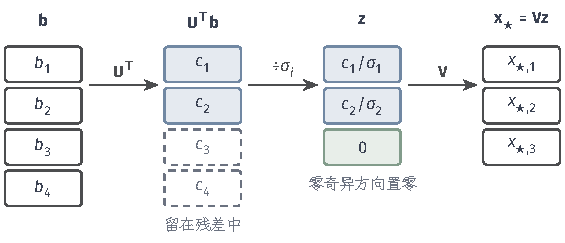
\includegraphics[width=95.652mm]{figures/01-basic-mathematics/03-vectors-matrices-and-multivariate-functions/tikz/c5-svd-solve-coordinates/figure.pdf}
  \caption{SVD求解的坐标变换，示意$m=4$、$d=3$、$r=2$。右端先变到左奇异坐标，蓝色的前$r$个坐标可以拟合，虚线框中的其余坐标无论怎样选$\bm x$都留在残差中；可拟合坐标除以对应奇异值，零奇异方向的坐标取零；最后由右奇异向量还原为原变量。}
  \label{fig:ls-svd-solve-coordinates}
\end{figure}

\subsubsection{算法实现}

输入$\bm A\in\mathbb R^{m\times d}$与$\bm b\in\mathbb R^m$，不要求满秩，输出最小范数最小二乘解$\bm x_\star$，没有额外超参数。这里按精确的正奇异值描述求解；有限精度下怎样判定数值秩，以及是否截断小奇异值，分别在第~\ref{sec:ls-pseudoinverse-rank-change}节和第~\ref{sec:ls-tsvd-solve}节讨论。

\paragraph{计算SVD}
第一步调用数值SVD过程，按第~\ref{sec:ls-svd}节的形式取得$\bm A=\bm U_r\bm\Sigma_r\bm V_r^\top$。其中$r=\operatorname{rank}\bm A$，$\bm U_r=[\bm u_1,\ldots,\bm u_r]$与$\bm V_r=[\bm v_1,\ldots,\bm v_r]$的列标准正交，$\bm\Sigma_r=\operatorname{diag}(\sigma_1,\ldots,\sigma_r)$且各$\sigma_i>0$。若$\bm A=\bm0$，则直接取$\bm x_\star=\bm0$并结束。

\paragraph{投影右端}
然后计算$\bm c=\bm U_r^\top\bm b$，即$c_i=\bm u_i^\top\bm b$，$i=1,\ldots,r$。这一步把右端投影到能够拟合的输出方向上；$\bm b$在其余方向上的部分，无论怎样选$\bm x$都会留在残差中。

\paragraph{按奇异值缩放}
接着对每个$i=1,\ldots,r$计算$z_i=c_i/\sigma_i$，得到产生这些输出所需的输入坐标。除法只对正奇异值进行，零奇异值对应的方向不参与。

\paragraph{还原原变量}
最后计算
\[
 \bm x_\star=\bm V_r\bm z=\sum_{i=1}^r\frac{\bm u_i^\top\bm b}{\sigma_i}\bm v_i
\]
并输出，把奇异坐标还原为原变量。整个过程只用到因子对向量的作用，无需形成完整的伪逆。

\begin{example}[秩一矩阵的SVD求解]
\label{ex:ls-svd-solve-rank-one}
取$\bm A=\left[\begin{smallmatrix}1&1\\1&1\end{smallmatrix}\right]$、$\bm b=(1,3)^\top$，方程不相容。$\bm A$的秩为$1$，$\sigma_1=2$，$\bm u_1=\bm v_1=(1,1)^\top/\sqrt2$。投影得$c_1=\bm u_1^\top\bm b=2\sqrt2$，缩放得$z_1=c_1/\sigma_1=\sqrt2$，还原得$\bm x_\star=z_1\bm v_1=(1,1)^\top$。核对：拟合值$\bm A\bm x_\star=(2,2)^\top$，残差$(-1,1)^\top$与列空间方向$(1,1)^\top$正交，长度$\sqrt2$等于$\bm b$在$\bm u_2=(1,-1)^\top/\sqrt2$上的分量的绝对值；$\bm x_\star$与核方向$(1,-1)^\top$正交。全部最小二乘解为$(1+t,1-t)^\top$，其中$t=0$时范数最小。
\end{example}

\subsubsection{算法分析}

\paragraph{正确性}
上述四步算出的正是伪逆作用于右端的结果。

\begin{theorem}[SVD求解给出\texorpdfstring{$\bm A^\dagger\bm b$}{A+b}]
\label{thm:ls-svd-solve}
对任意$\bm A\in\mathbb R^{m\times d}$与$\bm b\in\mathbb R^m$，上述过程的输出$\bm x_\star=\bm A^\dagger\bm b$，它是唯一的最小范数最小二乘解。
\end{theorem}
\begin{proof}
由式~\eqref{eq:matrix-analysis-pseudoinverse}，$\bm A^\dagger\bm b=\sum_{i\leq r}\bm v_i\bm u_i^\top\bm b/\sigma_i$，与输出相同；$\bm A=\bm0$时两者都是$\bm0$。最优性由定理~\ref{thm:matrix-analysis-pseudoinverse-minimum-norm}给出。也可以直接验证：残差$\bm b-\bm A\bm x_\star=\bm b-\bm U_r\bm U_r^\top\bm b$与列空间正交，所以$\bm x_\star$满足正规方程；$\bm x_\star\in\operatorname{range}(\bm V_r)=(\ker\bm A)^\perp$，由定理~\ref{thm:ls-minimum-norm-representative}，它在全部最小二乘解中范数最小。
\end{proof}

\paragraph{数值敏感度}
敏感性来自除以小奇异值。固定$\bm A$且$r>0$时，右端扰动$\delta\bm b$使解改变$\sum_{i=1}^r(\bm u_i^\top\delta\bm b)\bm v_i/\sigma_i$，其长度至多为$\lVert\delta\bm b\rVert_2/\sigma_r$，即放大倍数至多为$1/\sigma_r$。若为了压低放大而截去真实的正奇异值，求的就已不是$\bm A^\dagger\bm b$，这属于第~\ref{sec:ls-tsvd-solve}节的截断SVD。

\subsubsection{加权最小二乘}

加权问题的核心做法是把权矩阵写成$\bm M=\bm R^\top\bm R$，用同一个$\bm R$变换$\bm A$和$\bm b$，再求普通最小二乘。输入$\bm A$、$\bm b$，超参数是对称正定的权矩阵$\bm M\in\mathbb R^{m\times m}$，它规定目标函数为$(\bm A\bm x-\bm b)^\top\bm M(\bm A\bm x-\bm b)$；输出加权最小二乘解中欧氏范数最小的代表$\bm x_\star$。

\paragraph{构造权因子}
第一步构造权因子。用第~\ref{sec:ls-cholesky}节的方法作Cholesky分解$\bm M=\bm L\bm L^\top$，取$\bm R=\bm L^\top$；对角权$\bm M=\operatorname{diag}(w_1,\ldots,w_m)$则直接取$\bm R=\operatorname{diag}(\sqrt{w_1},\ldots,\sqrt{w_m})$。若权以$\bm M=\bm C^{-1}$的形式给出，就改为分解$\bm C=\bm L\bm L^\top$，这时$\bm M=\bm L^{-\top}\bm L^{-1}$，取$\bm R=\bm L^{-1}$，它的作用在下一步用前代实现。

\paragraph{白化数据}
然后计算$\widetilde{\bm A}=\bm R\bm A$和$\widetilde{\bm b}=\bm R\bm b$。在$\bm M=\bm C^{-1}$的形式下，对$\bm A$的各列和$\bm b$用前代求解$\bm L\widetilde{\bm A}=\bm A$与$\bm L\widetilde{\bm b}=\bm b$，不显式求逆。

\paragraph{求解普通最小二乘}
最后对$(\widetilde{\bm A},\widetilde{\bm b})$调用上面的SVD求解过程，得到$\bm x_\star$并输出；$\widetilde{\bm A}$满列秩时也可以调用第~\ref{sec:ls-qr-method}节的QR求解。变换只作用于观测端，未知量的坐标没有改变，无须另做恢复。

\begin{example}[两种权重下的白化求解]
\label{ex:ls-weighted-whitening-solve}
沿用示例~\ref{ex:linear-algebra-weighted-projection}的$\bm A=(1,1)^\top$、$\bm b=(2,1)^\top$、$\bm M=\operatorname{diag}(1,4)$。对角权直接取$\bm R=\operatorname{diag}(1,2)$，白化得$\widetilde{\bm A}=(1,2)^\top$、$\widetilde{\bm b}=(2,2)^\top$。$\widetilde{\bm A}$只有一列，QR因子为$\bm q=(1,2)^\top/\sqrt5$、$r=\sqrt5$，于是$c_1=\bm q^\top\widetilde{\bm b}=6/\sqrt5$，回代得$x_\star=c_1/r=6/5$，与该示例中加权正规方程$5a=6$的解一致。
\end{example}

\paragraph{正确性与数值敏感度}
由第~\ref{sec:ls-weighted-ls}节，变换前后的目标函数逐点相等，即$(\bm A\bm x-\bm b)^\top\bm M(\bm A\bm x-\bm b)=\lVert\widetilde{\bm A}\bm x-\widetilde{\bm b}\rVert_2^2$；未知量及其欧氏范数也没有变，所以两个问题的最优解集与最小范数代表都相同（定理~\ref{thm:ls-weighted-least-squares}）。数值敏感度取决于$\widetilde{\bm A}=\bm R\bm A$而不是$\bm A$：权重可能改善条件，也可能使它变差，应在变换后的系统上判断。

\subsubsection{齐次最小二乘}

齐次最小二乘的核心做法是在$\lVert\bm x\rVert_2=1$的约束下，选择被$\bm A$伸缩得最小的方向。它是$\bm b=\bm0$的特例，实际只依赖$\bm A$：输入$\bm A\in\mathbb R^{m\times d}$，没有额外超参数，输出使$\lVert\bm A\bm x\rVert_2$最小的单位向量$\hat{\bm x}$。单位长度约束属于求解目标，用来排除无意义的零解。

\paragraph{计算完整右奇异基}
第一步调用数值SVD过程，取得第~\ref{sec:ls-svd}节中的完整右因子$\bm V=[\bm v_1,\ldots,\bm v_d]$，各列按对应的伸缩量$\lVert\bm A\bm v_i\rVert_2$从大到小排列。$m<d$时奇异值只有$m$个，完整右基中多出的方向属于零空间，伸缩量记为零，也要保留。这些方向直接从$\bm A$的SVD取得，不通过显式形成$\bm A^\top\bm A$再求特征向量。

\paragraph{取最小方向}
然后取$\hat{\bm x}=\bm v_d$并输出。它已经是单位向量，无须再归一化。最小伸缩量重复时，$\bm v_d$只是最优子空间中的一个选择；$\hat{\bm x}$与$-\hat{\bm x}$表示同一组参数比例。

\paragraph{正确性与数值敏感度}
正确性直接来自定理~\ref{thm:ls-homogeneous-minimizers}：$\lVert\bm A\bm x\rVert_2^2=\bm x^\top\bm A^\top\bm A\bm x$在单位球面上的最小值是$\bm A^\top\bm A$的最小特征值，由对应的特征向量达到，而$\bm v_d$正是这样的向量。最优方向的敏感度由最小特征值与其余谱之间的间隙控制，可用第~\ref{sec:ls-subspace-sensitivity}节的子空间扰动界估计；最小特征值重复时，不能保证单个方向唯一。单位长度与最优性的检验按第~\ref{sec:ls-least-squares-verification}节进行。

\subsection{直接求解的选择与核验}
\label{sec:ls-direct-method-comparison}

选择回到第~\ref{sec:ls-solution-selection}节确定的求解目标。求精确解时，非奇异方阵用LU，对称正定矩阵用Cholesky，对称不定矩阵用分块LDL。求最小二乘解时，满列秩用QR，条件数适中时也可用正规方程法；满行秩欠定方程的最小范数解用转置QR；一般秩的情形用SVD。已知块结构时，先用被消块的分解得到Schur补方程，再恢复其余分量（第~\ref{sec:ls-block-elimination}节）；系数只作低秩修改时，复用旧矩阵的分解，只多解一个小系统（第~\ref{sec:ls-woodbury}节）。这两种做法都不是新的分解，而是复用上面的求解步骤。

在同一组数据上比较几条路线。沿用示例~\ref{ex:ls-line-least-squares}的直线拟合$\bm A=\left[\begin{smallmatrix}1&0\\1&1\\1&2\end{smallmatrix}\right]$、$\bm b=(1,2,2)^\top$。正规方程法形成$\bm G=\left[\begin{smallmatrix}3&3\\3&5\end{smallmatrix}\right]$与$\bm c=(5,6)^\top$，Cholesky因子为$\bm L=\left[\begin{smallmatrix}\sqrt3&0\\\sqrt3&\sqrt2\end{smallmatrix}\right]$，前代得$\bm y=(5/\sqrt3,1/\sqrt2)^\top$，回代得$\hat{\bm x}=(7/6,1/2)^\top$。QR路线得到$\bm R=\bm L^\top$与$\bm c_1=\bm y$，回代出同一个$\hat{\bm x}$：两条路线解的是同一个三角方程，只是得到它的方式不同。复制常数列后得到$\widetilde{\bm A}=\left[\begin{smallmatrix}1&0&1\\1&1&1\\1&2&1\end{smallmatrix}\right]$，列空间和最优残差都不变，但秩降为$2$，正规方程与QR回代都会遇到零主元。SVD求解略去$\sigma_3=0$对应的方向$(1,0,-1)^\top/\sqrt2$，得到最小范数解$\bm x_\star=(7/12,1/2,7/12)^\top$。前两条路线的差别在计算方式，这里的差别则在选解目标。

算出$\bm x$后，代回原问题检查它是否符合目标：精确解检查$\bm A\bm x=\bm b$，普通最小二乘解检查$\bm A^\top(\bm b-\bm A\bm x)=\bm0$，要求最小范数时再检查$\bm x\perp\ker\bm A$。在上例中，残差$(-\tfrac16,\tfrac13,-\tfrac16)^\top$不为零，但它与$\bm A$的两列都正交；$\widetilde{\bm A}\bm x_\star=\bm A\hat{\bm x}$，且$\bm x_\star$与核方向$(1,0,-1)^\top$正交。加权问题使用第~\ref{sec:ls-least-squares-verification}节的加权正交条件，齐次问题检查单位长度以及是否为最小特征方向。最小二乘的残差本来就可以非零；这些量用于核对计算过程和示例，各求解算法仍只返回$\bm x$。

计算中可以用分解的重构误差（如$\lVert\bm A-\bm Q_1\bm R\rVert$）和正交性（如$\lVert\bm Q_1^\top\bm Q_1-\bm I\rVert$）分别核对中间变换，但这些检查只是旁证，不属于算法本身。残差小也不保证$\bm x$的误差小：矩阵接近奇异时，很小的残差可能对应很大的解误差。第~\ref{sec:ls-numerical-sensitivity}节用条件数与前向、后向误差解释这一差别，与迭代法的整体比较留到第~\ref{sec:ls-method-selection}节。
